% Sinh tự động bởi report/scripts/ve_hinh_bitboard.py, đừng sửa tay.
\definecolor{bbX}{HTML}{1F4E8C}
\definecolor{bbO}{HTML}{C8553D}
\definecolor{bbKq}{HTML}{2E8B57}
\definecolor{bbSai}{HTML}{D7263D}
\definecolor{bbMat}{HTML}{DCE8F5}
\definecolor{bbVang}{HTML}{FBE7A1}
\definecolor{bbXam}{HTML}{BDBDBD}
\definecolor{bbNhat}{HTML}{9CC3E6}
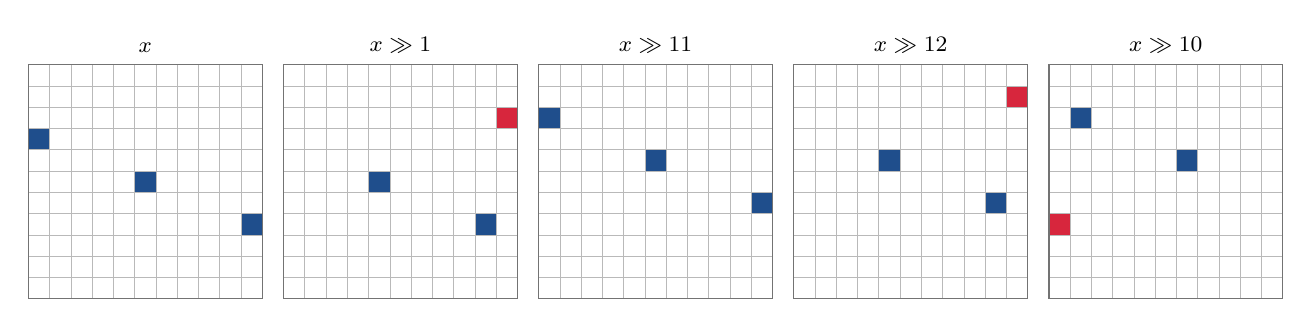
\begin{tikzpicture}
\begin{scope}[shift={(0.000,0.000)}]
\fill[bbX] (0.000,-0.810) rectangle ++(0.270,-0.270);
\fill[bbX] (1.350,-1.350) rectangle ++(0.270,-0.270);
\fill[bbX] (2.700,-1.890) rectangle ++(0.270,-0.270);
\draw[gray!55,line width=.2pt] (0,0) grid[step=0.270] (2.970,-2.970);
\draw[gray!90!black,line width=.5pt] (0,0) rectangle (2.970,-2.970);
\node[anchor=south,font=\footnotesize] at (1.485,0.03) {$x$};
\end{scope}
\begin{scope}[shift={(3.240,0.000)}]
\fill[bbX] (1.080,-1.350) rectangle ++(0.270,-0.270);
\fill[bbX] (2.430,-1.890) rectangle ++(0.270,-0.270);
\fill[bbSai] (2.700,-0.540) rectangle ++(0.270,-0.270);
\draw[gray!55,line width=.2pt] (0,0) grid[step=0.270] (2.970,-2.970);
\draw[gray!90!black,line width=.5pt] (0,0) rectangle (2.970,-2.970);
\node[anchor=south,font=\footnotesize] at (1.485,0.03) {$x \gg 1$};
\end{scope}
\begin{scope}[shift={(6.480,0.000)}]
\fill[bbX] (0.000,-0.540) rectangle ++(0.270,-0.270);
\fill[bbX] (1.350,-1.080) rectangle ++(0.270,-0.270);
\fill[bbX] (2.700,-1.620) rectangle ++(0.270,-0.270);
\draw[gray!55,line width=.2pt] (0,0) grid[step=0.270] (2.970,-2.970);
\draw[gray!90!black,line width=.5pt] (0,0) rectangle (2.970,-2.970);
\node[anchor=south,font=\footnotesize] at (1.485,0.03) {$x \gg 11$};
\end{scope}
\begin{scope}[shift={(9.720,0.000)}]
\fill[bbX] (1.080,-1.080) rectangle ++(0.270,-0.270);
\fill[bbX] (2.430,-1.620) rectangle ++(0.270,-0.270);
\fill[bbSai] (2.700,-0.270) rectangle ++(0.270,-0.270);
\draw[gray!55,line width=.2pt] (0,0) grid[step=0.270] (2.970,-2.970);
\draw[gray!90!black,line width=.5pt] (0,0) rectangle (2.970,-2.970);
\node[anchor=south,font=\footnotesize] at (1.485,0.03) {$x \gg 12$};
\end{scope}
\begin{scope}[shift={(12.960,0.000)}]
\fill[bbX] (0.270,-0.540) rectangle ++(0.270,-0.270);
\fill[bbX] (1.620,-1.080) rectangle ++(0.270,-0.270);
\fill[bbSai] (0.000,-1.890) rectangle ++(0.270,-0.270);
\draw[gray!55,line width=.2pt] (0,0) grid[step=0.270] (2.970,-2.970);
\draw[gray!90!black,line width=.5pt] (0,0) rectangle (2.970,-2.970);
\node[anchor=south,font=\footnotesize] at (1.485,0.03) {$x \gg 10$};
\end{scope}
\end{tikzpicture}
